%% FullCourse_10Lecs -- Lecture 8, Act 8.2 (INDEX): Chunking and Embeddings.
%% Rebuilt 2026-07-08 per Lec08_Rewrite_Plan_2026-07-08.md ("one map, five acts").
%% Source: archive_pre_split/pre_map_rebuild_2026-07-08/Lec08_T2_RAG_Chunking_Embeddings.tex
%% (23 frames -> 16; the three near-duplicate architecture diagrams consolidated
%% into one pipeline anchor, pooling/contrastive mechanics reduced to intuition,
%% appendix table dropped, broken wiki-demo checkpoint replaced by a corrected
%% pointer in the Bridge closer).

%% Shared preamble for the FullCourse_10Lecs topic decks.
%%
%% Each topic .tex \input's this file, then defines its own \title, \date
%% override (if any), \graphicspath, and \begin{document}.
%%
%% Reconstructed verbatim from the inlined copy preserved in
%% Lec10_Case_Studies/Lec10_T8_Case6_DeepRamsey.tex (lines 23-190), which is
%% explicitly annotated there as "from ../shared_preamble.tex, copied verbatim".
%% Base preamble matches MiniCourse_8hr/Slides/shared_preamble.tex; this version
%% additionally provides \sectiondivider, the conceptbox/cautionbox/examplebox/
%% takeawaybox tcolorboxes, and \compacttables used across the split decks.

\documentclass[10pt,english,aspectratio=169]{beamer}

\usepackage{ae,aecompl}
\usepackage[T1]{fontenc}
\usepackage{textcomp}
\usepackage[utf8]{inputenc}
\usepackage{babel}
\usepackage{datetime2}

\setcounter{secnumdepth}{3}
\setcounter{tocdepth}{3}

\usepackage{amsmath, amssymb, amsthm, graphicx}
\usepackage{booktabs, multirow}
\usepackage{tikz}
\usepackage{pgfplots}
\pgfplotsset{compat=1.16}
\usepackage[most]{tcolorbox}
\tcbuselibrary{skins, breakable, theorems}
\usepackage{listings}
\usepackage{xcolor}

\lstset{
  basicstyle=\ttfamily\small,
  keywordstyle=\color{blue!80!black}\bfseries,
  commentstyle=\color{green!50!black}\itshape,
  stringstyle=\color{orange!80!black},
  backgroundcolor=\color{gray!8},
  frame=single,
  rulecolor=\color{gray!40},
  breaklines=true,
  showstringspaces=false,
  numbers=none,
}

\lstdefinestyle{pythonstyle}{
    language=Python,
    basicstyle=\ttfamily\footnotesize,
    keywordstyle=\color{blue!80!black}\bfseries,
    commentstyle=\color{green!50!black}\itshape,
    stringstyle=\color{orange!80!black},
    frame=single,
    breaklines=true,
    showstringspaces=false,
    numbers=left,
    numbersep=5pt,
    numberstyle=\tiny\color{gray},
    backgroundcolor=\color{gray!8},
    rulecolor=\color{gray!40}
}

\ifx\hypersetup\undefined
  \AtBeginDocument{%
    \hypersetup{bookmarks=false,breaklinks=true,pdfborder={0 0 0},colorlinks=true,
      linkcolor=DarkText,urlcolor=RedTitle}%
  }
\else
  \hypersetup{bookmarks=false,breaklinks=true,pdfborder={0 0 0},colorlinks=true,
    linkcolor=DarkText,urlcolor=RedTitle}%
\fi

\makeatletter
\newcommand\makebeamertitle{%
  \begin{frame}[plain]
    \vspace*{1.0cm}
    \centering
    {\usebeamerfont{title}\usebeamercolor[fg]{title}\inserttitle\par}
    \vspace{1.0cm}
    {\usebeamerfont{author}\usebeamercolor[fg]{author}\insertauthor\par}
    \vspace{0.2cm}
    {\usebeamerfont{date}\usebeamercolor[fg]{date}\insertdate\par}
  \end{frame}}%
\AtBeginDocument{%
  \let\origtableofcontents=\tableofcontents
  \def\tableofcontents{\@ifnextchar[{\origtableofcontents}{\gobbletableofcontents}}
  \def\gobbletableofcontents#1{\origtableofcontents}%
}

\usetheme{metropolis}
\usefonttheme{professionalfonts}

\definecolor{LightGray}{RGB}{230,230,230}
\definecolor{RedTitle}{RGB}{0,0,200}
\definecolor{VeryLightGray}{RGB}{245,245,245}
\definecolor{DarkText}{RGB}{0,0,0}

\setbeamercolor{background canvas}{bg=white}
\setbeamercolor{title}{fg=RedTitle}
\setbeamercolor{author}{fg=DarkText}
\setbeamercolor{date}{fg=DarkText}
\setbeamercolor{frametitle}{bg=VeryLightGray,fg=DarkText}
\setbeamercolor{normal text}{fg=DarkText}
\setbeamerfont{title}{size=\large}

\setbeamersize{text margin left=5mm, text margin right=5mm}
\addtobeamertemplate{frametitle}{}{\vspace{-0.5em}}
\newcommand{\reducevspace}{\vspace{-0.5cm}}

% Shared section divider and box styles for split topic decks.
\newcommand{\sectiondivider}[2]{%
\begin{frame}[plain,noframenumbering]
\begin{center}
\vfill
{\Large\textbf{#1}\par}
\vspace{0.35cm}
{\normalsize #2\par}
\vfill
\end{center}
\end{frame}
}

\newtcolorbox{conceptbox}[1][]{
  colback=blue!3,
  colframe=RedTitle!55,
  boxrule=0.35mm,
  arc=1mm,
  left=2mm,
  right=2mm,
  top=1mm,
  bottom=1mm,
  #1
}
\newtcolorbox{cautionbox}[1][]{
  colback=red!3,
  colframe=red!50!black,
  boxrule=0.35mm,
  arc=1mm,
  left=2mm,
  right=2mm,
  top=1mm,
  bottom=1mm,
  #1
}
\newtcolorbox{examplebox}[1][]{
  colback=green!3,
  colframe=green!45!black,
  boxrule=0.35mm,
  arc=1mm,
  left=2mm,
  right=2mm,
  top=1mm,
  bottom=1mm,
  #1
}
\newtcolorbox{takeawaybox}[1][]{
  colback=VeryLightGray,
  colframe=RedTitle!55,
  boxrule=0.35mm,
  arc=1mm,
  left=2mm,
  right=2mm,
  top=1mm,
  bottom=1mm,
  #1
}
\newcommand{\compacttables}{\renewcommand{\arraystretch}{1.15}}

\setbeamertemplate{navigation symbols}{}
\setbeamertemplate{footline}{%
  \hfill%
  \usebeamercolor[fg]{page number in head/foot}%
  \usebeamerfont{page number in head/foot}%
  \insertframenumber\,/\,\inserttotalframenumber\kern1em\vskip2pt%
}

\makeatother

\author{Zhigang Feng}
% "date with time": compile timestamp so each build is identifiable.
\date{\today\ \DTMcurrenttime}

\metroset{sectionpage=none}

\usetikzlibrary{arrows.meta, positioning, shapes, shapes.geometric, fit, calc, backgrounds}

\graphicspath{{./pic/}{./figures/}{../../MiniCourse_8hr/Slides/Module4_Agentic_AI/pic/}{../}}

%% Lec08 shared MAP slide: "one map, five acts" recurring diagram.
%% Adapted from ../Lec07_LLM/lec07_map.tex (\LecSevenMap -> \LecEightMap).
%% Input this file AFTER ../shared_preamble.tex (needs RedTitle, VeryLightGray)
%% and call \LecEightMap{k} inside a frame, where k in {1..5} highlights the
%% current act ("you are here") and k = 0 renders the closing reprise with all
%% five acts complete (used by T5's closing frame).
%% Filename deliberately does not match the build glob Lec*_T*.tex, so the
%% build script never tries to compile it standalone.

\newcommand{\LecEightMap}[1]{%
% Precompute per-box style selectors; TikZ option lists are comma-split before
% TeX conditionals run, so \ifnum must not sit inside a [...] options list.
\ifnum#1=0
  \tikzset{lecmapa/.style={lecmapdone}, lecmapb/.style={lecmapdone},
           lecmapc/.style={lecmapdone}, lecmapd/.style={lecmapdone},
           lecmape/.style={lecmapdone}}%
\else
  \tikzset{lecmapa/.style={}, lecmapb/.style={}, lecmapc/.style={},
           lecmapd/.style={}, lecmape/.style={}}%
  \ifnum#1=1 \tikzset{lecmapa/.style={lecmapcur}}\fi
  \ifnum#1=2 \tikzset{lecmapb/.style={lecmapcur}}\fi
  \ifnum#1=3 \tikzset{lecmapc/.style={lecmapcur}}\fi
  \ifnum#1=4 \tikzset{lecmapd/.style={lecmapcur}}\fi
  \ifnum#1=5 \tikzset{lecmape/.style={lecmapcur}}\fi
\fi
\begin{center}
\begin{tikzpicture}[
    act/.style={rectangle, rounded corners, draw=black!60, fill=VeryLightGray,
        minimum width=2.6cm, minimum height=0.92cm, text width=2.5cm,
        align=center, font=\scriptsize, text=DarkText},
    lecmapcur/.style={draw=RedTitle, very thick, fill=orange!20},
    lecmapdone/.style={draw=green!45!black, thick, fill=green!10},
    q/.style={font=\tiny\itshape, text width=2.7cm, align=center, text=black!70},
    sat/.style={rectangle, rounded corners, draw=black!45, dashed, fill=white,
        text width=5.0cm, align=center, font=\tiny, text=black!70,
        minimum height=0.5cm},
    barlab/.style={font=\tiny\bfseries, text=black!60},
    arr/.style={-{Stealth[length=2mm]}, thick, gray!60}
]
    % --- five act boxes ---
    \node[act, lecmapa] (a1) at (0,0)
        {\textbf{8.1 WALL}\\ \tiny naive prompting fails};
    \node[act, lecmapb] (a2) at (2.85,0)
        {\textbf{8.2 INDEX}\\ \tiny chunk \& embed once};
    \node[act, lecmapc] (a3) at (5.7,0)
        {\textbf{8.3 RETRIEVE}\\ \tiny vector, hybrid, graph};
    \node[act, lecmapd] (a4) at (8.55,0)
        {\textbf{8.4 GENERATE}\\ \tiny cited, refusable answers};
    \node[act, lecmape] (a5) at (11.4,0)
        {\textbf{8.5 APPLY}\\ \tiny corpora, demo, evaluation};
    \draw[arr] (a1) -- (a2);
    \draw[arr] (a2) -- (a3);
    \draw[arr] (a3) -- (a4);
    \draw[arr] (a4) -- (a5);
    % --- the student question each act answers ---
    \node[q] at (0,-0.82)    {why not just paste\\ it all in?};
    \node[q] at (2.85,-0.82) {how does my corpus\\ become searchable?};
    \node[q] at (5.7,-0.82)  {how does the right\\ passage come back?};
    \node[q] at (8.55,-0.82) {how do I get citations,\\ not hallucinations?};
    \node[q] at (11.4,-0.82) {what does this change\\ for my research?};
    % --- "you are here" marker above the current act ---
    \ifnum#1=1 \node[font=\scriptsize\bfseries, text=RedTitle] at (0,0.95)
        {you are here\ $\blacktriangledown$};\fi
    \ifnum#1=2 \node[font=\scriptsize\bfseries, text=RedTitle] at (2.85,0.95)
        {you are here\ $\blacktriangledown$};\fi
    \ifnum#1=3 \node[font=\scriptsize\bfseries, text=RedTitle] at (5.7,0.95)
        {you are here\ $\blacktriangledown$};\fi
    \ifnum#1=4 \node[font=\scriptsize\bfseries, text=RedTitle] at (8.55,0.95)
        {you are here\ $\blacktriangledown$};\fi
    \ifnum#1=5 \node[font=\scriptsize\bfseries, text=RedTitle] at (11.4,0.95)
        {you are here\ $\blacktriangledown$};\fi
    \ifnum#1=0 \node[font=\scriptsize\bfseries, text=green!45!black] at (5.7,0.95)
        {all five acts complete};\fi
    % --- bottom band: problem / pipeline / payoff ---
    \fill[blue!10]   (-1.3,-1.55) rectangle (1.40,-1.22);
    \fill[green!10]  (1.65,-1.55) rectangle (9.85,-1.22);
    \fill[orange!15] (10.1,-1.55) rectangle (12.7,-1.22);
    \node[barlab] at (0.05,-1.385) {THE PROBLEM};
    \node[barlab] at (5.75,-1.385) {THE PIPELINE};
    \node[barlab] at (11.4,-1.385) {YOUR RESEARCH};
    % --- the recurring spine (the RAG pipeline), printed under the band ---
    \node[font=\tiny\itshape, text=black!60] at (5.7,-1.83)
        {the pipeline:\ \ corpus $\to$ chunk $\to$ embed $\to$ index
         \;$\big\|$\; query $\to$ retrieve $\to$ augment $\to$ cited answer};
    % --- dashed satellites: the neighbouring lectures ---
    \node[sat] at (2.0,-2.42)
        {\textit{before 8.1:} Lec07 gave you the language engine --- frozen
         weights, finite context; RAG is its grounded memory};
    \node[sat] at (9.8,-2.42)
        {\textit{after 8.5:} Lec09 agents --- retrieval becomes one tool the
         model chooses to call $\to$ Lec10 cases};
\end{tikzpicture}
\end{center}
}


\title[AI for Econ Research]{AI for Economic Research: Dynamic Models, Language, and Agents\\
Lecture 8.2: Index --- Chunking and Embeddings}

\begin{document}

\makebeamertitle

%=============================================================================
\begin{frame}{Map: Act 8.2 --- Build the Index}
\textbf{Act 1 hit the wall. Act 2 builds the machine's offline half: the index.}
\LecEightMap{2}
\textit{\footnotesize Route this deck: one pipeline picture $\to$ chunking (what is a retrieval unit?) $\to$ embeddings (text becomes geometry).
Thread A: the FOMC minutes get chunked and embedded here; Thread B: the same recipe indexes the OLG literature in Acts 8.3 and 8.5.}
\end{frame}

%=============================================================================
\section{RAG: The Principled Solution}
\sectiondivider{RAG: The Principled Solution}{Index once, query many}

\begin{frame}{The Key Insight: Index Once, Query Many}
\textbf{Don't paste the whole corpus into every prompt --- pre-process it once, then fetch only what each question needs.}

\medskip
\begin{itemize}
\item \textbf{The recipe:}
\begin{enumerate}
    \item \textbf{Pre-process documents once.} Split them into chunks, convert each chunk to a numerical fingerprint (an \emph{embedding}), store everything in a database.
    \item \textbf{At query time, fetch only what's relevant.} Convert the question to an embedding, look up the closest chunks, paste \emph{those few chunks} into the prompt.
    \item \textbf{Let the LLM answer from the retrieved evidence}, citing which chunks it used.
\end{enumerate}

\medskip
\item \textbf{A two-phase architecture:} \emph{offline}, index everything once; \emph{online}, retrieve a few relevant pieces per query and generate.

\medskip
\item Cost is now proportional to \emph{what you actually need}, not to the size of the corpus. Storage is amortized; indexes are updatable; the model only ever sees relevant text, so quality and faithfulness improve.
\end{itemize}
\end{frame}

\begin{frame}{The Whole Pipeline in One Picture}
\textbf{The machine for the rest of the lecture --- offline index built once, online loop run thousands of times.}
\begin{center}
\begin{tikzpicture}[
  font=\footnotesize,
  node distance=0.45cm and 0.6cm,
  off/.style={draw, rounded corners=2pt, minimum width=1.85cm, minimum height=0.5cm, align=center, fill=blue!7},
  on/.style={draw, rounded corners=2pt, minimum width=1.85cm, minimum height=0.5cm, align=center, fill=orange!12},
  store/.style={draw, cylinder, shape border rotate=90, aspect=0.25, minimum width=1.7cm, minimum height=0.9cm, align=center, fill=blue!10},
  arr/.style={-{Latex[length=2.0mm]}, thick}
]
  % Top row: Offline Phase
  \node[font=\footnotesize\bfseries, anchor=west] at (-0.3, 1.85) {Offline (do once; the index = institutional memory)};
  \node[off] (docs)   at (0.5, 1.2) {Collect\\(PDF, HTML)};
  \node[off] (chunk)  at (3.2, 1.2) {Chunk\\(+ metadata)};
  \node[off] (emb1)   at (5.9, 1.2) {Embed\\(transformer)};
  \node[store] (db)   at (8.8, 0.25) {Vector\\Store};
  \draw[arr] (docs) -- (chunk);
  \draw[arr] (chunk) -- (emb1);
  \draw[arr] (emb1.east) -- ++(0.5,0) |- (db.north);

  % Bottom row: Online Phase
  \node[font=\footnotesize\bfseries, anchor=west] at (-0.3, -0.45) {Online (do every query; cheap, cached, audit-friendly)};
  \node[on] (q)       at (0.5, -1.1) {User\\Query};
  \node[on] (emb2)    at (3.2, -1.1) {Embed\\(same model)};
  \node[on] (retr)    at (5.9, -1.1) {Top-$K$\\Retrieve};
  \node[on] (gen)     at (8.8, -1.1) {Augmented\\Generate};
  \node[on] (ans)     at (11.6, -1.1) {Cited\\Answer};
  \draw[arr] (q) -- (emb2);
  \draw[arr] (emb2) -- (retr);
  \draw[arr] (db.south) |- (retr.west);
  \draw[arr] (retr) -- (gen);
  \draw[arr] (gen) -- (ans);

  % Visual separator
  \draw[gray, dashed] (-0.5, 0.3) -- (12.5, 0.3);
\end{tikzpicture}
\end{center}

\textit{\footnotesize Five parts: \textbf{chunker} + \textbf{embedder} (this act) $\to$ \textbf{vector store} + \textbf{retriever} (8.3) $\to$ \textbf{prompt} + \textbf{generator} (8.4).}

\smallskip
\begin{cautionbox}
\textbf{One rule already:} use the \emph{same embedder} for indexing and queries --- otherwise the geometries don't line up.
\end{cautionbox}
\end{frame}

\begin{frame}{Definition and Origin}
\textbf{Retrieval Augmented Generation (RAG): before answering, \emph{retrieve} relevant documents from an external store and supply them to the model as context for \emph{generation}.}

\medskip
\begin{itemize}
\item \textbf{Origin:} Lewis, Perez, Piktus, et al.\ (2020), ``Retrieval-Augmented Generation for Knowledge-Intensive NLP Tasks,'' \emph{NeurIPS}.

\medskip
\item Originally a research architecture for open-domain QA. Now the \emph{de facto} production pattern for any LLM application over a custom knowledge base: customer support, legal research, medical Q\&A, code search --- and academic research.

\medskip
\item \textbf{Key idea (worth repeating):} the LLM is the \emph{reasoner}. The vector store is the \emph{memory}. The retriever is the \emph{librarian}. RAG is how we connect them.
\end{itemize}
\end{frame}

%=============================================================================
\section{Chunking}
\sectiondivider{Chunking}{What is a retrieval unit?}

\begin{frame}{Why Chunk At All?}
\textbf{Documents are too big to embed as a single vector --- the corpus must be split into retrieval units first.}

\medskip
\begin{itemize}
\item \textbf{Three reasons to chunk:}
\begin{enumerate}
    \item \textbf{Embedder input limits.} Most embedding models accept 512--8192 tokens per input. A 60-page FOMC transcript blows past every limit.
    \item \textbf{Granularity of relevance.} Index a 30-page document as one vector and the embedding averages over many topics --- the \emph{one paragraph} on inflation expectations disappears into the mean.
    \item \textbf{Generator context budget.} Only a few chunks go into the prompt. Smaller chunks $\Rightarrow$ more chunks fit $\Rightarrow$ richer evidence base.
\end{enumerate}

\medskip
\item \textbf{Trade-off:} chunks too large $\Rightarrow$ noisy embeddings; too small $\Rightarrow$ context lost.
\end{itemize}

\medskip
\begin{takeawaybox}
\emph{Choosing the chunking strategy is the most consequential decision in a RAG pipeline.}
\end{takeawaybox}
\end{frame}

\begin{frame}{Chunking Strategies: The Cost--Quality Trade-Off}
\textbf{One rule governs the menu: better retrieval costs more parsing effort} --- the five common strategies line up along that single trade-off.

\vspace{-1mm}
\begin{center}
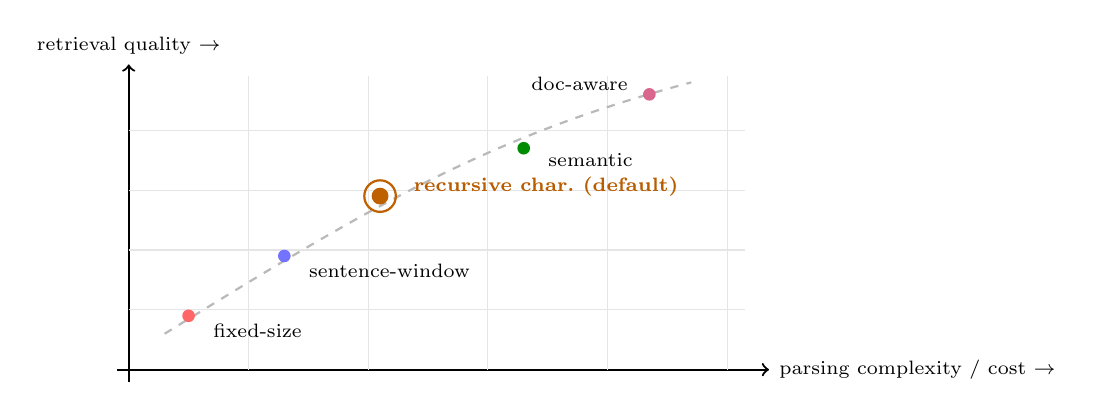
\begin{tikzpicture}[font=\scriptsize, scale=0.76]
  % axes
  \draw[->, thick] (-0.2,0) -- (10.7,0) node[right, font=\scriptsize] {parsing complexity / cost $\to$};
  \draw[->, thick] (0,-0.2) -- (0,5.1) node[above, font=\scriptsize] {retrieval quality $\to$};
  % light gridlines
  \foreach \x in {2,4,6,8,10} \draw[gray!20] (\x,0) -- (\x,4.9);
  \foreach \y in {1,2,3,4} \draw[gray!20] (0,\y) -- (10.3,\y);

  % the trade-off frontier (more cost -> more quality, diminishing returns)
  \draw[gray!55, thick, dashed] (0.6,0.6) .. controls (4,2.7) and (6,3.9) .. (9.4,4.8);

  % strategy points, ordered along the frontier (x = cost, y = retrieval quality)
  \fill[red!60]          (1.0,0.9) circle (3pt);
  \node[anchor=west] at (1.25,0.65) {fixed-size};

  \fill[blue!55]         (2.6,1.9) circle (3pt);
  \node[anchor=west] at (2.85,1.65) {sentence-window};

  % recursive = recommended default (highlighted)
  \fill[orange!75!black] (4.2,2.9) circle (4pt);
  \draw[orange!75!black, thick] (4.2,2.9) circle (7.5pt);
  \node[anchor=west, font=\scriptsize\bfseries, orange!72!black] at (4.6,3.05) {recursive char.\ (default)};

  \fill[green!55!black]  (6.6,3.7) circle (3pt);
  \node[anchor=west] at (6.85,3.5) {semantic};

  \fill[purple!60]       (8.7,4.6) circle (3pt);
  \node[anchor=east] at (8.5,4.78) {doc-aware};
\end{tikzpicture}
\end{center}

\vspace{-2mm}
{\footnotesize \textbf{Read it as a frontier:} more effort $\to$ higher retrieval quality, with diminishing returns. \textbf{Rule of thumb:} start at \emph{recursive character} (LangChain's default); climb to \emph{document-aware} for richly structured corpora (FOMC, 10-K), and to \emph{semantic} only when recursive retrieval is \emph{measurably} noisy. Chunk \emph{size} and \emph{overlap} are separate knobs, tuned next.}
\end{frame}

\begin{frame}{Fixed-Size vs.\ Recursive: An FOMC Example}
\textbf{The same paragraph, two chunkers --- one destroys meaning, one preserves it.}

\smallskip
\begin{itemize}
\item \textbf{Source paragraph} (FOMC minutes, simplified):
\begin{quote}
\small\itshape
``Participants observed that inflation remained elevated. Several noted that core services prices, especially shelter, continued to rise. A few participants expressed concern about persistence in wage growth. Most agreed that policy should remain restrictive.''
\end{quote}

\smallskip
\item \textbf{Fixed 60-character chunks:}
\begin{quote}
\small\ttfamily
{[}``Participants observed that inflation remained elevat''] \\
{[}``ed. Several noted that core services prices, especi''] \dots
\end{quote}
$\Rightarrow$ \textbf{Cuts mid-word.} Embeddings of these fragments are nearly useless.

\smallskip
\item \textbf{Recursive chunking} (split on paragraph $\to$ sentence $\to$ word, target $\sim$120 chars):
\begin{quote}
\small\ttfamily
[``Participants observed that inflation remained elevated.''] \\
{[}``Several noted that core services prices, especially shelter, continued to rise.'']
\end{quote}
$\Rightarrow$ Each chunk is a self-contained sentence. Embeddings carry meaning.
\end{itemize}
\end{frame}

\begin{frame}[fragile]{Practical Defaults + Code}
\textbf{Three defaults cover most projects:} chunk size 500--1000 tokens ($\sim$2--4 paragraphs); overlap 10--20\%; \textbf{always preserve metadata} --- doc ID, page, section, date, author.

\smallskip
\begin{lstlisting}[language=Python]
from langchain.text_splitter import RecursiveCharacterTextSplitter

splitter = RecursiveCharacterTextSplitter(
    chunk_size=800,            # ~600 tokens
    chunk_overlap=100,         # ~80 tokens of overlap
    separators=["\n\n", "\n", ". ", " ", ""],
)

chunks = splitter.create_documents(
    texts=[fomc_minutes_text],
    metadatas=[{"meeting": "2024-06", "doc_type": "minutes"}],
)
\end{lstlisting}
\end{frame}

\begin{frame}{The Economist's Chunking Gotcha}
\textbf{Real institutional documents have structure that generic chunkers destroy --- and the structure is exactly what you will want to filter on later.}

\medskip
\begin{itemize}
\item \textbf{FOMC minutes:} organized as \emph{speaker turns} (``Participants generally agreed\dots'', ``A few members noted\dots''). Cutting across speaker boundaries fuses unrelated viewpoints.

\medskip
\item \textbf{Congressional Record:} hierarchical metadata --- Congress / session / chamber / date / speaker / bill. Lose the hierarchy and you can't filter or cite properly.

\medskip
\item \textbf{SEC 10-K filings:} standardized item numbers (Item 1, Item 1A Risk Factors, Item 7 MD\&A). A query about ``risk factors'' should retrieve only \emph{Item 1A} content --- which only works if you parse the structure first.

\medskip
\item \textbf{Practical fix:} write a corpus-specific parser that emits chunks with rich metadata. Extra effort up front; a large payoff in retrieval quality and filtering (Act 8.3 uses exactly this metadata).
\end{itemize}

\medskip
\begin{takeawaybox}
Don't reach for the generic chunker. \textbf{Let your corpus tell you what a chunk should be.}
\end{takeawaybox}
\end{frame}

%=============================================================================
\section{Embeddings}
\sectiondivider{Embeddings}{Text becomes geometry}

\begin{frame}{From Text to Vectors: What and Why}
\textbf{An embedding turns a piece of text into a point in space --- and turns ``find relevant passages'' into geometry.}

\medskip
\begin{itemize}
\item An \textbf{embedding} is a function $E: \text{text} \to \mathbb{R}^d$ mapping text to a fixed-length vector; typical $d \in \{384, 768, 1024, 1536, 3072\}$.

\medskip
\item \textbf{The crucial property:}
\[
\text{semantically similar texts } \;\Longrightarrow\; \text{nearby vectors in } \mathbb{R}^d
\]

\medskip
\item \textbf{Why this is useful:} once the corpus lives in a vector space, ``find documents about inflation expectations'' becomes \emph{nearest-neighbor search} around the query's embedding.

\medskip
\item \textbf{Callback:} Lec.\ 7 T3b (``Token Embeddings vs.\ Document Embeddings --- Bridge to Lec08'') showed token embeddings living \emph{inside} the transformer. Here a separate \emph{retrieval-tuned} model produces one vector per \emph{chunk}.
\end{itemize}
\end{frame}

\begin{frame}{Geometric Intuition: Trained So Similar Texts Land Nearby}
\begin{center}
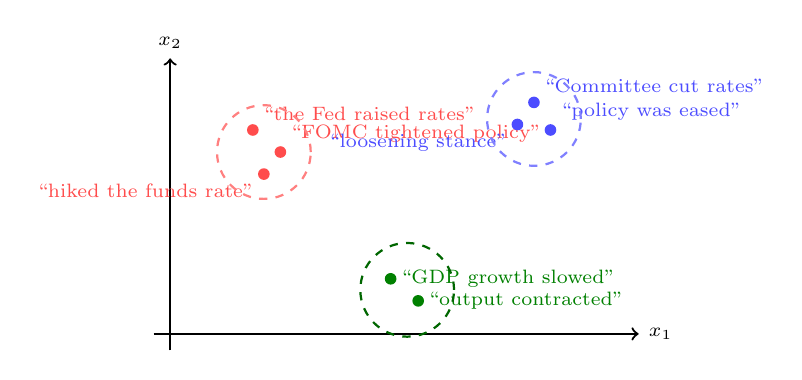
\begin{tikzpicture}[font=\scriptsize, scale=0.70]
  \draw[->, thick] (-0.3,0) -- (8.5,0) node[right] {$x_1$};
  \draw[->, thick] (0,-0.3) -- (0,5.0) node[above] {$x_2$};

  % Cluster A: hawkish / tightening
  \fill[red!70] (1.5,3.7) circle (3pt) node[above right, font=\scriptsize] {``the Fed raised rates''};
  \fill[red!70] (2.0,3.3) circle (3pt) node[above right, font=\scriptsize] {``FOMC tightened policy''};
  \fill[red!70] (1.7,2.9) circle (3pt) node[below left, font=\scriptsize] {``hiked the funds rate''};
  \draw[red!50, thick, dashed] (1.7,3.3) circle (0.85);

  % Cluster B: dovish / easing
  \fill[blue!70] (6.6,4.2) circle (3pt) node[above right, font=\scriptsize] {``Committee cut rates''};
  \fill[blue!70] (6.9,3.7) circle (3pt) node[above right, font=\scriptsize] {``policy was eased''};
  \fill[blue!70] (6.3,3.8) circle (3pt) node[below left, font=\scriptsize] {``loosening stance''};
  \draw[blue!50, thick, dashed] (6.6,3.9) circle (0.85);

  % Cluster C: unrelated
  \fill[green!50!black] (4.0,1.0) circle (3pt) node[right, font=\scriptsize] {``GDP growth slowed''};
  \fill[green!50!black] (4.5,0.6) circle (3pt) node[right, font=\scriptsize] {``output contracted''};
  \draw[green!40!black, thick, dashed] (4.3,0.8) circle (0.85);
\end{tikzpicture}
\end{center}

\smallskip
\begin{itemize}
\item Hawkish clusters left; dovish right; growth talk elsewhere. \textbf{Distance in vector space $\approx$ distance in meaning} --- ``find me speeches like this one'' becomes nearest-neighbor search under cosine (the hook Lec.\ 7 T2b planted).

\smallskip
\item \textbf{Why it works:} a retrieval embedder is a transformer encoder \emph{pooled} to one vector per text and \emph{trained contrastively} --- similar pairs pulled together, unrelated pushed apart --- so the geometry is learned for similarity. \textit{\footnotesize Sentence-BERT lineage: Reimers \& Gurevych (2019); mechanics in Lec.\ 7 T3b.}
\end{itemize}
\end{frame}

\begin{frame}{Choosing an Embedder (mid-2026)}
\textbf{Four models cover a researcher's realistic day-one choices --- pick by hosting constraint, not leaderboard decimals.}

\medskip
\begin{center}
\renewcommand{\arraystretch}{1.3}
\small
\begin{tabular}{|l|c|l|l|}
\hline
\textbf{Model} & \textbf{Dim} & \textbf{Access} & \textbf{Why pick it} \\
\hline
OpenAI \texttt{text-embedding-3-small} & 1536 & API (metered) & cheap default, no infra \\
\hline
OpenAI \texttt{text-embedding-3-large} & 3072 & API (metered) & top accuracy, paid \\
\hline
\texttt{voyage-3} & 1024 & API (metered) & top retrieval benchmarks \\
\hline
\texttt{bge-large-en-v1.5} & 1024 & local (free) & best open-source default \\
\hline
\end{tabular}
\end{center}

\smallskip
{\centering\textit{\footnotesize Model facts current as of mid-2026.}\par}

\medskip
\textbf{For an academic researcher:}
\begin{itemize}
\item \textbf{Local + free:} \texttt{bge-large-en-v1.5} --- runs on a laptop GPU; competitive with paid APIs.
\item \textbf{Cloud + simple:} \texttt{text-embedding-3-small} --- metered but inexpensive, zero infrastructure.
\item \textbf{Top accuracy with budget:} \texttt{voyage-3} or \texttt{text-embedding-3-large}.
\end{itemize}
\end{frame}

\begin{frame}{Economists' Embedding Example: Fed Chair Speeches}
\textbf{Embed every Fed Chair speech 2010--2025, project to 2D, and the policy eras separate --- with no labels supplied.}

\medskip
\begin{itemize}
\item \textbf{The setup.} Embed each speech (Bernanke, Yellen, Powell) with \texttt{bge-large-en-v1.5}; project to 2D with UMAP; plot.

\medskip
\item \textbf{What you see:}
\begin{itemize}
    \item Crisis-era Bernanke (2010--2014) clusters together --- QE, financial stability.
    \item Normalization-era Yellen (2015--2017) forms a distinct cluster --- gradual exit, forward guidance.
    \item Powell splits in two: 2020--2021 dovish ``patient'' speeches vs.\ 2022--2024 hawkish ``restrictive'' speeches.
\end{itemize}

\medskip
\item \textbf{Why this matters for research:} the clustering comes \emph{purely from the text}. The economist gains a reproducible measure of stance shifts, linkable to rate decisions, market reactions, or macro outcomes.

\medskip
\item \textit{\footnotesize Sources in this literature: Hansen, McMahon \& Prat (2018, QJE) --- FOMC transcripts; Shapiro \& Wilson (2021, REStat) --- Fed sentiment; Gentzkow, Kelly \& Taddy (2019, JEL) --- text-as-data survey.}
\end{itemize}
\end{frame}

\begin{frame}{The Domain-Adaptation Problem}
\textbf{Generic embedders learned English from the open web --- they did not learn Fed English.}

\medskip
\begin{itemize}
\item \textbf{Where they struggle:}
\begin{itemize}
    \item ``\emph{patient}'' in a Fed statement = \emph{dovish} --- a domain code word.
    \item CUSIP codes, BEA NIPA tables, FRED series IDs --- alphanumeric strings with no web-English meaning.
    \item ``Section 13(3)'', ``LSAP'' --- technical citations the embedder has rarely seen.
\end{itemize}

\medskip
\item \textbf{Two fixes:}
\begin{enumerate}
    \item \textbf{Fine-tune the embedder} on a domain corpus --- a few GPU-hours (\texttt{sentence-transformers}, \texttt{MultipleNegativesRankingLoss}), real quality gains.
    \item \textbf{Hybrid retrieval} (Act 8.3): combine dense embeddings with classical sparse retrieval (BM25), which catches the exact-match queries the embedder misses.
\end{enumerate}

\medskip
\item \textbf{In practice:} hybrid is cheaper and gets you 80\% of the gain. Fine-tune only when retrieval quality is demonstrably your bottleneck.
\end{itemize}
\end{frame}

\begin{frame}[fragile]{Code: Embed FOMC Chunks}
\begin{lstlisting}[language=Python, basicstyle=\ttfamily\footnotesize]
from sentence_transformers import SentenceTransformer

# 1. Load a strong open-source embedder
model = SentenceTransformer("BAAI/bge-large-en-v1.5")

# 2. Suppose `chunks` is a list of FOMC chunk strings
chunks = [
    "Participants observed that inflation remained elevated.",
    "Several noted that core services prices continued to rise.",
    # ... thousands more
]

embeddings = model.encode(   # one numpy vector per chunk
    chunks,
    batch_size=32,
    normalize_embeddings=True,   # so cosine sim = dot product
)

print(embeddings.shape)  # (N_chunks, 1024) -- ready for the store
\end{lstlisting}
\end{frame}

\begin{frame}{Bridge: The Corpus Is Now Geometry}
\textbf{Act 2 built the offline half: chunks that respect the corpus's structure, carrying metadata, each with a learned vector.}

\medskip
\begin{itemize}
\item \textbf{Three load-bearing decisions made here:} chunk strategy (recursive vs.\ document-aware), embedder choice (open-source vs.\ API), domain adaptation (hybrid first; fine-tune only if retrieval bottlenecks).

\medskip
\item \textbf{Hands-on, two scales:} browse \texttt{wiki\_demo/} (Act 8.1's manual wiki --- markdown articles + an index, no retriever); then preview \texttt{demos/M4\_rag\_olg\_demo} --- a runnable \emph{TF-IDF} retriever over an OLG survey paper, the sparse cousin of today's embeddings. Full classroom run in Act 8.5.

\medskip
\item \textbf{Next --- Act 8.3 (RETRIEVE):} where the vectors live and how the right passage comes back --- vector databases, similarity search, hybrid dense+sparse, metadata filters, and what to do when similarity alone is not enough (GraphRAG).
\end{itemize}

\bigskip
\centering
\footnotesize\textit{Arc: Act 1 WALL $\to$ \textbf{Act 2 INDEX} $\to$ Act 3 RETRIEVE $\to$ Act 4 GENERATE $\to$ Act 5 APPLY.}
\end{frame}

\end{document}
